Lõputöö analüütiline osa peab sisaldama visiooni kirjeldust ja skoobi
määramist põhjendusega. Metoodikat, kuidas kõige edukamalt lõpptulemuseni
jõuda. Missuguseid võimalusi on teada selle probleemi lahendamiseks. Määrata
funktsionaalsed ja mittefunktsionaalsed tingimused. Selle alusel kirjeldada
kasutajalood või siis teha tegevuse plokkskeem. Leida töövahendid
põhjendatult: milliste kriteeriumite alusel tuleb valik teha, milline lahendus
valitakse selle töö puhul, kindlasti põhjendada.
Analüüs peab sisaldama vastuseid küsimustele:
\begin{enumerate}
    \item visiooni kirjeldust ja skoobi määramist põhjendusega
    \item missuguseid lahendusi te teate oma probleemi lahendamiseks
    \item milliste kriteeriumite alusel tuleb valik teha
    \item millise lahenduse valisite teie ja põhjendage seda
\end{enumerate}



\section{Nõuete defineerimine}
Nõuete määramisel lähtutakse erinevate osapoolte vajadusest - süsteemi kasutaja (klient) ja süsteemi administraator (tooteomanik).


\textbf{Süsteemi kasutajana tahan:}
\begin{itemize}
    \item registreerida endale konto ja logida sisse
    \item logida sisse
    \item hallata oma konto andmeid
    \item tellida tasulist paketi
    \item vaadata enda poolt salvestatud materjalide nimekirja
    \item luua ja salvestada uus materjal
    \item redigeerida varem salvestatud materjal
    \item kustutada varem salvestatud materjal
    \item lisada uus kiht konstruktsiooni mudelisse
    \item valida uue kihi materjal
    \item sisestada uue kihi paksuse väärtust
    \item redigeerida olemasolevat kihti
    \item kustutada olemasolevat kihti
    \item vahetada kihtide järjekorda
    \item valida välistingimuste parameetrid
    \item valida sisetingimuste parameetrid
    \item valida konstruktsiooni tüüp
    \item vaadata tulemusi tabeli kujul (valikuliselt)
    \item vaadata tulemusi graafikul (valikuliselt)
    \item vaadata konstruktsiooni toimivuse mõõdikuid
    \item peale igat muutust kohe näha uusi tulemusi (arvulised väärtused)
    \item peale igat muutust kohe näha graafikute uuendamist
    \item näha konstruktsiooni skemaatilist joonist
    \item salvestada mudeldatud konstruktsiooni
    \item vaadata salvestatud konstruktsioonid
    \item kustutada salvestatud konstruktsioonid
    \item avada salvestatud konstruktsioonid kalkulaatoris
    \item muuta kiht mittehomogeenseks
    \item mittehomogeensele kihile lisada alamkihid
    \item valida alamkihtide materjalid
    \item sisestada alamkihtide paksuse väärtust
    \item näha konstruktsiooni skemaatilist joonist
    \item näha skemaatilise joonise peal graafikut
    \item näha skemaatilise joonise peal värvilist temperatuurikaarti
    \item näha dünaamilist analüüsi aasta lõikes
    \item valida kliimaandmeid dünaamilise analüüsi jaoks
    \item genereerida analüüsi aruanne PDF formaadis
\end{itemize}

Kliendipoolsed kasutajalood on 

\begin{figure}[ht]
    \centering
    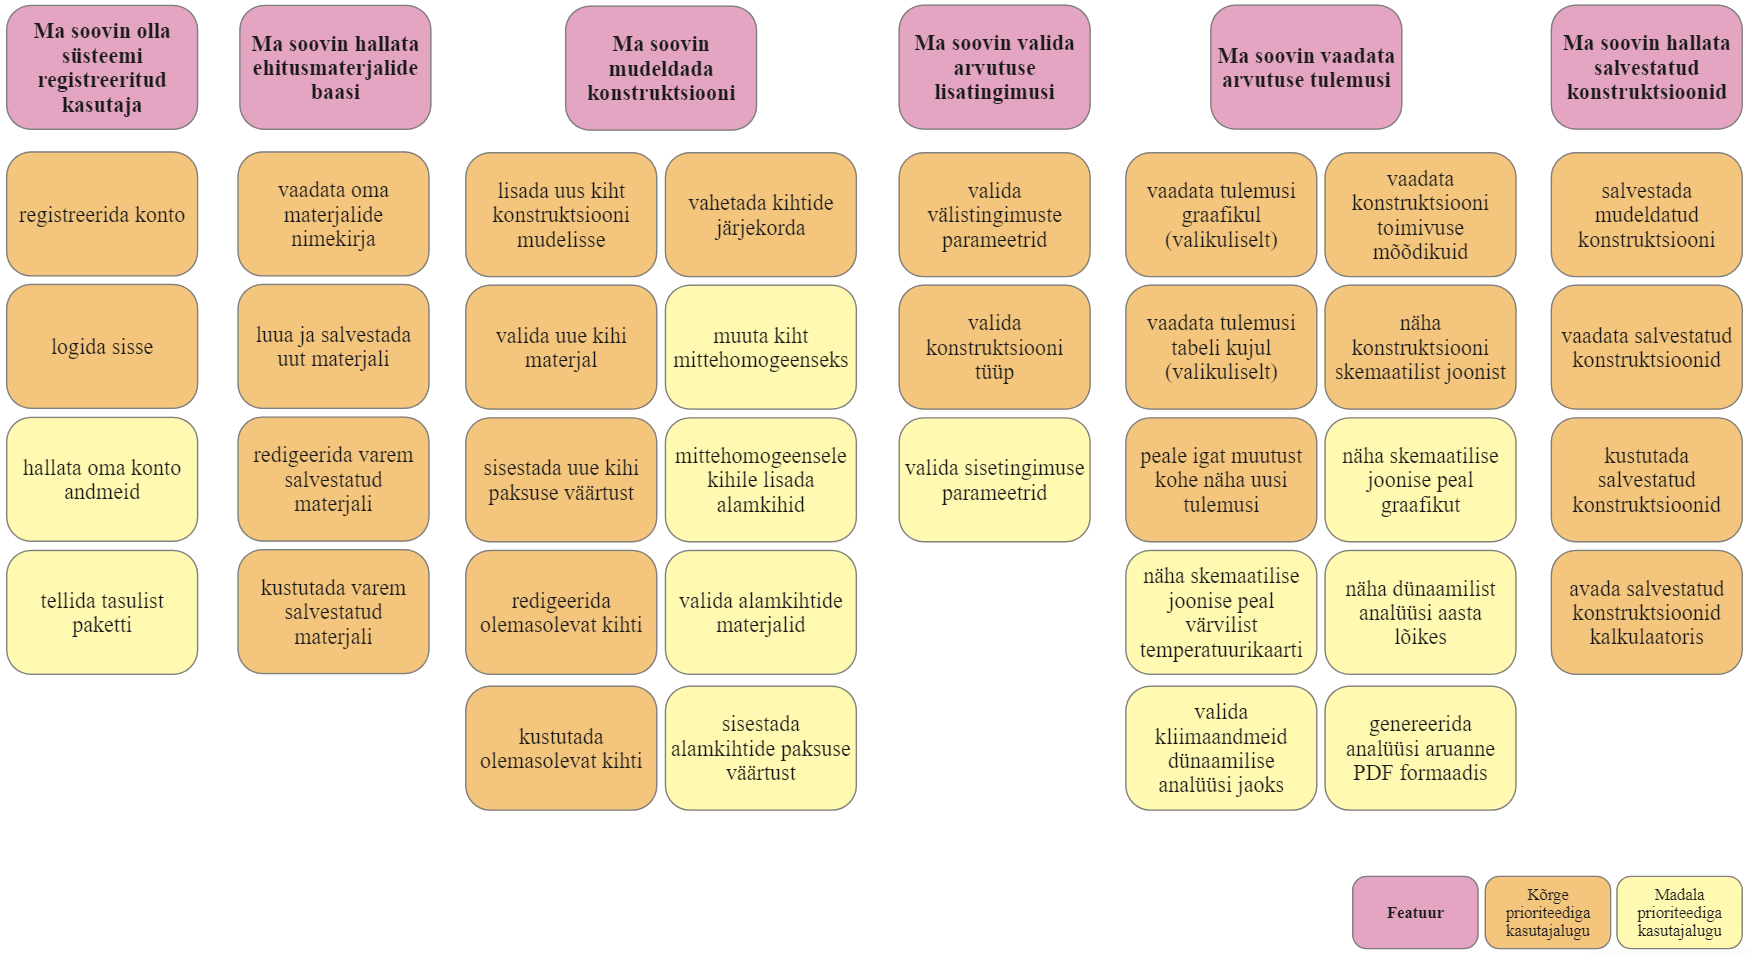
\includegraphics[width=1\textwidth]{figures/analysis/client_userstories.png}
    \caption[Funktsionaalsed nõuded, kliendi kasutajalood]{\textit{Kliendi kasutajalood}}
    \label{fig:client_userstories}
\end{figure}

\textbf{Infosüsteemi administraatorina soovin:}
\begin{itemize}

    \item vaadata kasutajate nimekirja
    \item hallata kasutajaid
    \item seadistada tellimust vormistanud kasutajale vastavad õigused
    \item hallata kasutajate andmeid
    \item vaadata süsteemis salvestatud vaikimisi materjalide nimekirja
    \item salvestada uus materjal
    \item määrata materjali ligipääsu taset
    \item redigeerida varem salvestatud materjal
    \item kustutada varem salvestatud materjal
    \item hallata uusi materjali kategooriaid
    \item hallata uusi materjalide tootjaid
    \item hallata keskkonna seadistuse valikuid
    \item lisada kliimaandmeid failina
\end{itemize}


\begin{figure}[ht]
    \centering
    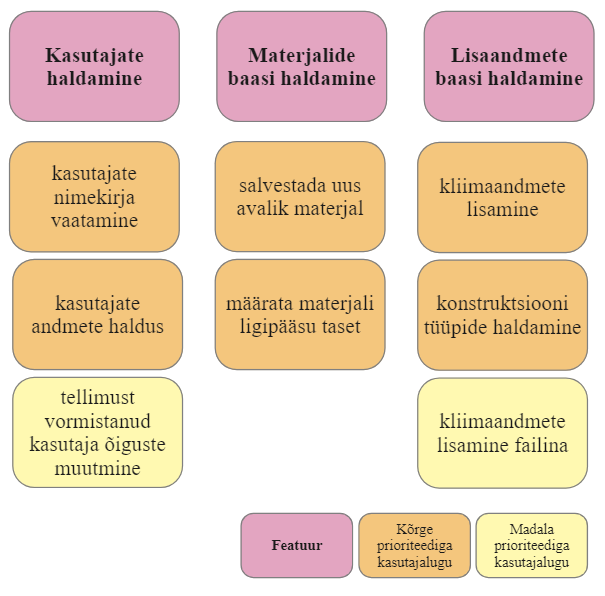
\includegraphics[width=0.6\textwidth]{figures/analysis/admin_userstories.png}
    \caption[Funktsionaalsed nõuded, administraatori kasutajalood]{\textit{administraatori kasutajalood}}
    \label{fig:admin_userstories}
\end{figure}


\section{Tehnoloogiate ja meetodite valik}
Osa, kus käsitletakse tehnoloogiaid ja arendusmetoodikate valikut.

\section{Veebirakenduse arhitektuur}
Osa, kus käsitletakse kavandatava rakenduse arhitektuuri planeerimist.

\section{Andmebaasi projekteerimine}
Osa, kus käsitletakse andmebaasi projekteerimist.

\section{Kasutajaliidese disain}
Osa, kus käsitletakse kasutajaliidest ja selle kavandamist